\startchapter{Channel Modeling}
\label{chapter:Mod}
In this section, I modeled communication in the traces. Then I investigated 4 different channel types: Named pipes, MQMS, TCP/UDP socket and HTTP channels, all of which are the most fundamental ones in Windows communication framework. By matching these channels to the communication model I verified generality of the modeling. 

\section{Communication Modeling}\label{commod}
As defined before, a communication event in the dual-trace is defined as message send and received in a specific channel. In the assembly trace level, we have to be able to locate the send or receive function calls of a specific channel in both side of the traces and then retrieve the message from the memory change recorded in the trace. 
\subsection{How Communications Happen}   
A communication in this work is happen in a channel. There are 3 main stages of a communication in this model: 1. open the channel, 2. message send/receive, 3. close the channel. Figure \ref{communicationhappen} indicate how communications happen between two ends of both sides of a channel. In the open channel stage, each end need to call its own channel open functions. This open function might be one or more functions which can be channel create function, open function, connect function etc.  In the message send/receive stage, messages are being sent into the channel in one side and received in the other side. In the final channel close stage, the channel delete function, disconnect function, close function etc. will be called. The channel can be reopen again to start new communications after the close stage. However the reopen channel will be treated as a communication cycle.

The operations being concerned in this model are: channel open in sender side, channel open in the receiver side, message send, message receive, channel close in sender side, channel close in receiver side. The number of send and receive function calls for one message do not necessary to be the same. It can be one to one, one to multiple, multiple to one, or multiple to multiple. Both sides of the channel shared the same channel name but different channel handle for its own operations.

\begin{figure}[h]
\centerline{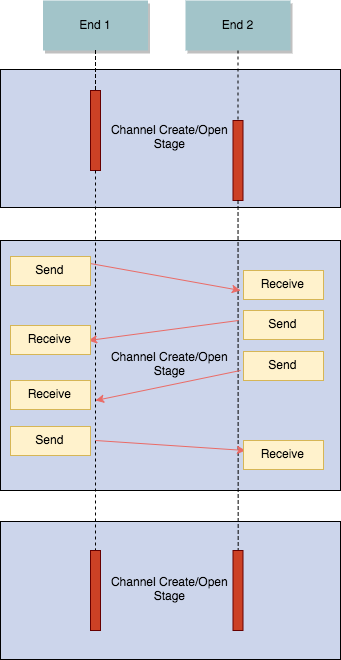
\includegraphics[scale=0.6]{Figures/communicationhappen}}
 \caption{Communication Model}
\label{communicationhappen}
\end{figure}

\subsection{Communication Scenarios}
This model contains several send/receive scenarios. Figure \ref{scenario1} to Figure \ref{scenario13} shows all of these scenarios.

\begin{figure}[ht!]
\centerline{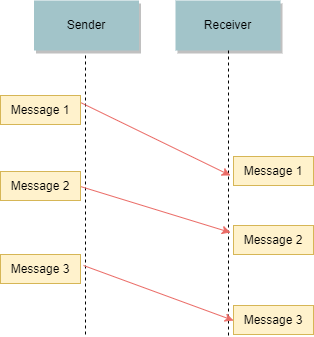
\includegraphics[scale=0.6]{Figures/scenario1}}
 \caption{Scenario 1: Message send/receive successfully in order}
\label{scenario1}
\end{figure}

\begin{figure}[ht!]
\centerline{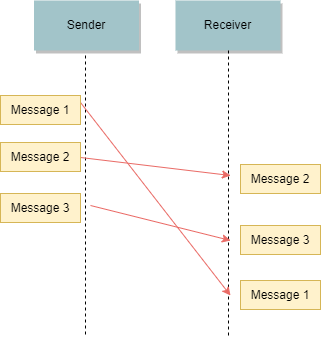
\includegraphics[scale=0.6]{Figures/scenario2}}
 \caption{Scenario 2: Message send/receive successfully but out of order}
\label{scenario2}
\end{figure}

\begin{figure}[ht!]
\centerline{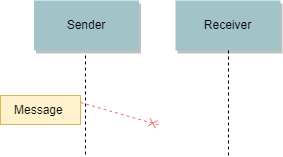
\includegraphics[scale=0.6]{Figures/scenario3}}
 \caption{Scenario 3: Message send/receive fail}
\label{scenario3}
\end{figure}

\begin{figure}[ht!]
\centerline{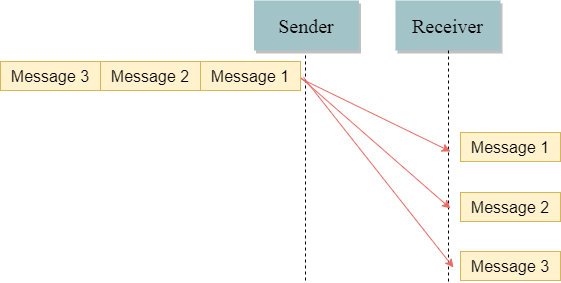
\includegraphics[scale=0.6]{Figures/scenario4}}
 \caption{Scenario 4: One sent message received segmented}
\label{scenario4}
\end{figure}

\begin{figure}[ht!]
\centerline{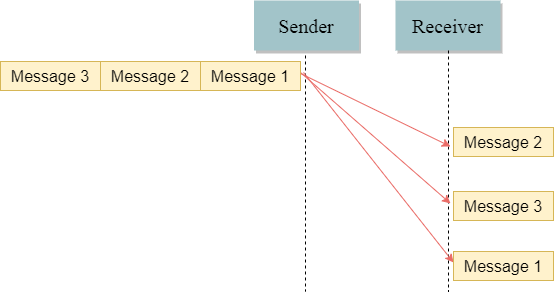
\includegraphics[scale=0.6]{Figures/scenario5}}
 \caption{Scenario 5: One sent message received segmented and out of order}
\label{scenario5}
\end{figure}

\begin{figure}[ht!]
\centerline{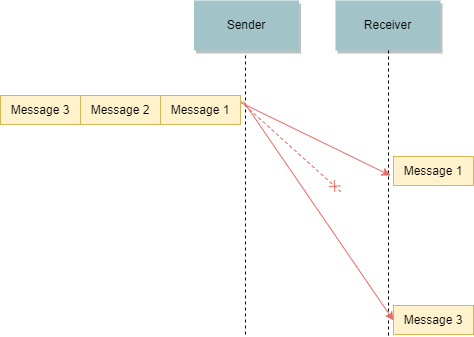
\includegraphics[scale=0.6]{Figures/scenario6}}
 \caption{Scenario 6: One sent message received segmented in order, but partially lost}
\label{scenario6}
\end{figure}

\begin{figure}[ht!]
\centerline{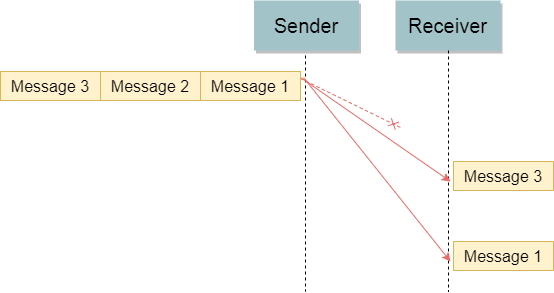
\includegraphics[scale=0.6]{Figures/scenario7}}
 \caption{Scenario 7: One sent message received segmented out of order and partially lost}
\label{scenario7}
\end{figure}

\begin{figure}[ht!]
\centerline{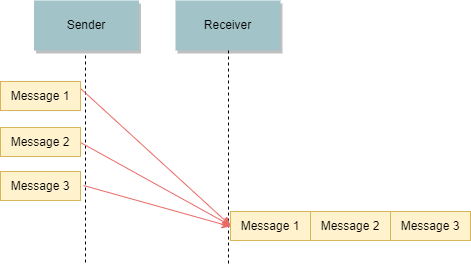
\includegraphics[scale=0.6]{Figures/scenario8}}
 \caption{Scenario 8: Multiple messages received at a time}
\label{scenario8}
\end{figure}

\begin{figure}[ht!]
\centerline{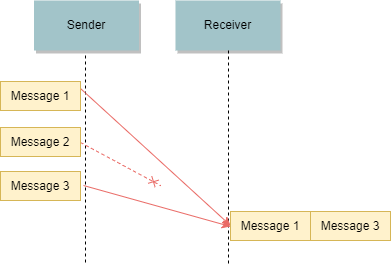
\includegraphics[scale=0.6]{Figures/scenario9}}
 \caption{Scenario 9: Multiple messages received at a time, but partially lost}
\label{scenario9}
\end{figure}

\begin{figure}[ht!]
\centerline{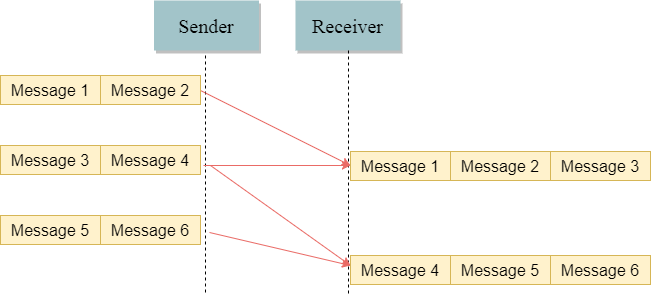
\includegraphics[scale=0.6]{Figures/scenario10}}
 \caption{Scenario 10: Messages segmented and reconstructed in order}
\label{scenario10}
\end{figure}

\begin{figure}[ht!]
\centerline{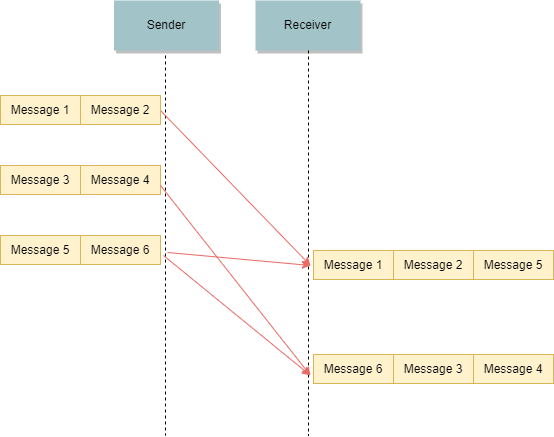
\includegraphics[scale=0.6]{Figures/scenario11}}
 \caption{Scenario 11: Messages segmented and reconstructed out of order}
\label{scenario11}
\end{figure}

\begin{figure}[ht!]
\centerline{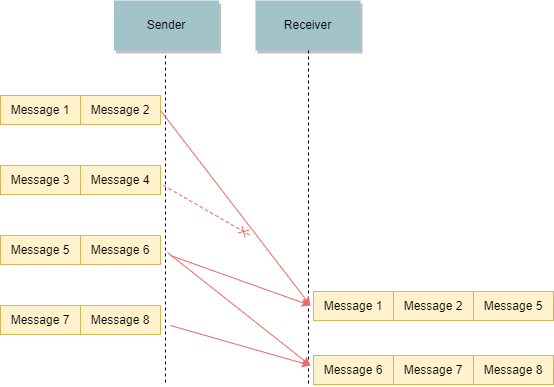
\includegraphics[scale=0.6]{Figures/scenario12}}
 \caption{Scenario 12: Messages segmented and reconstructed partially lost}
\label{scenario12}
\end{figure}
\clearpage
\begin{figure}[ht!]
\centerline{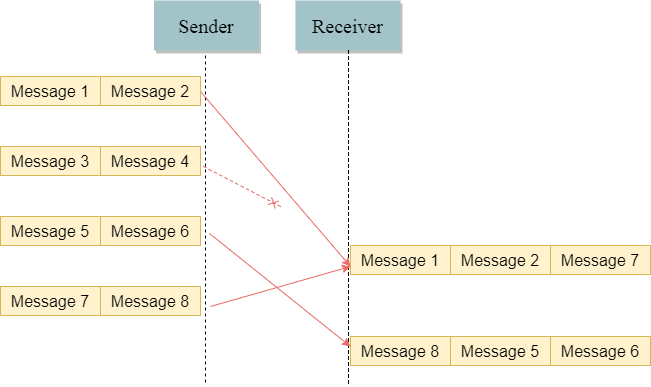
\includegraphics[scale=0.6]{Figures/scenario13}}
 \caption{Scenario 13: Messages segmented and reconstructed out of order and partially lost}
\label{scenario13}
\end{figure}

\section{Named Pipes Channel}
A named pipe is a named, one-way or duplex pipe for communication between the pipe server and one or more pipe clients. Both the server and client can read or write into the pipe. The pipe server and client can be on the same or different computers.  In here we only consider one server V.S one client dual-trace. One server to multiple clients scenario can always be divided into multiple server/client dual-traces. We call the end of the named pipe instance. An instance can be a server instance or a client instance. All instances of a named pipe share the same pipe name, but each instance has its own buffers and handles, and provides a separate conduit for client/server communication. 

A named pipe server responsible for the creation of the pipe, while clients of the pipe can connect to the server after it created. The creation and connection of a named pipe will return the handle ID of that pipe. As we mention before, each instance has its own handles, so the returned handle IDs of the pipe creation function of the server and pipe connection function from each client are different. These handler IDs will be used later on when messages are being sent or received to specify a pipe to which send.

\subsection{Important Channel Parameters}
There are many options for a named pipe. Some of them are critical in the perspective of the channel operations. In this sections we list the important ones.

\subsubsection{Blocking/Non-Blocking}
The named pipe channel can be opened in blocking mode or non-blocking mode. In blocking mode, when the pipe handle is specified in the ReadFile, WriteFile, or ConnectNamedPipe function, the operations are not completed until there is data to read, all data is written, or a client is connected. In non-blocking mode, ReadFile, WriteFile, and ConnectNamedPipe always return immediately. The operation fail if the channel is not ready for read, write or connection. However, since in this work we only aimed at locating the successful communication, as long as the operations success, we can locate them no matter the pipe is in blocking or non-blocking mode.

\subsubsection{Synchronous/Asynchronous}
Another critical option for named pipe channel is Synchronous/Asynchronous. In Synchronous mode, the ReadFile, WriteFile TracnsactNamedPipe and connectNamedPipe functions does not return until the operation it is performing is completed. That means we can retrieve the sent/receive message in the trace when the function return. When the channel is enable overlapped mode, the ReadFile, WriteFile TracnsactNamedPipe and connectNamedPipe functions perform asynchronously. In the asynchronous mode, ReadFile, WriteFile, TransactNamedPipe, and ConnectNamedPipe operations return immediately regardless if the operations are completed. And if the function call return ERROR\_IO\_PENDING, the calling thread then call the GetOverlappedResult function to determine the results. For the read operation, the message will be stored in the buffer indicated in the ReadFile function call when the read operation complete successfully.

\subsection{Send/Receive Scenarios}
In this section, I matched the possible send/receive scenarios of named pipe channel with those defined in the \ref{commod} section. The matching result is list in Table \ref{modmatchresult} with comments.

\begin{table}[h]
\centering
\caption{Send/Receive Scenarios of Named Pipe}
\label{modmatchresult}
\begin{tabular}{|l|l|l|}
\hline
\begin{tabular}[c]{@{}l@{}}\textbf{Scenario} \end{tabular} & \begin{tabular}[c]{@{}l@{}}\textbf{Existence}\end{tabular} & \begin{tabular}[c]{@{}l@{}}\textbf{Comment}\end{tabular}\\ \hline
Scenario 1 & YES & The most basic scenario                       \\ \hline
Scenario 2 & NO  & All message going into the pipe will go out in order                                         \\ \hline
Scenario 3 & YES & Message write or read fail                                                 \\ \hline
Scenario 4 & YES & The sent message size larger than the reader's read buffer                                           \\ \hline
Scenario 5 & NO  & All message going into the pipe will go out in order                                         \\ \hline
Scenario 6 & NO  & Same as Scenario 5 \\ \hline
Scenario 7 & NO  & Same as Scenario 5 \\ \hline
Scenario 8 & NO  & The reader can only read content from a write on the other side of the pipe.                                                 \\ \hline
Scenario 9 & NO  & Same as Scenario 8                                                 \\\hline
Scenario 10 & NO &   Same as Scenario 8                                               \\ \hline
Scenario 11 & NO &  Same as Scenario 8                                                 \\ \hline
Scenario 12 & NO &  Same as Scenario 8                                                 \\ \hline
Scenario 13 & NO & Same as Scenario 8                                                  \\ \hline
\end{tabular}
\end{table}


\begin{figure}[h]
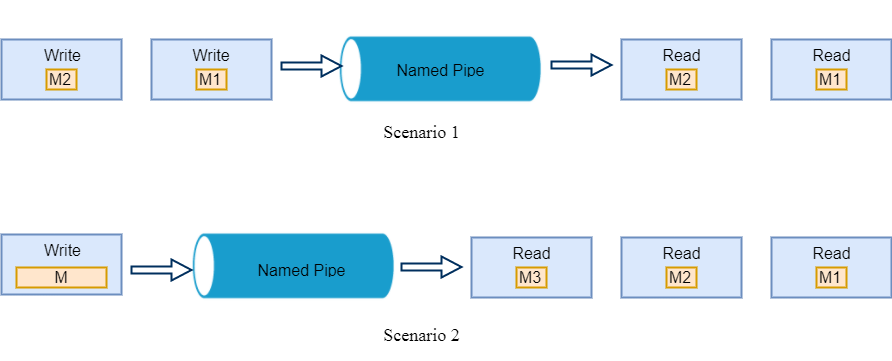
\includegraphics[scale=.48]{Figures/event}
 \caption{Two successful write/read operation scenarios. Each blue block indicate a single read or write operation.}
\label{event}
\end{figure}


\subsection{Function Calls In Each Communication Stage}
As we talk in the parameters section, Synchrounous and Asychronous mode affect the functions used to complete the send and receive operation as well as the operation of the functions. In the follow subsections, we will list the related functions for the named pipe channel for both synchronous mode and asynchronous mode. The create channel functions for both modes are the same but with different input parameters. The functions for send and receive message are also the same for both case. However, the operation of the send and receive functions are different for different mode. In addition, extra functions are being called to check the status of message sending or receiving in asynchronous mode.
\subsubsection{Synchronous}
We list all the functions that needed to locate an messaging event in a dual-trace in Table\ref{synfunctions} for synchronous named pipe. The Channel Create Functions indicate how the channel being created in server and client sides, and they are different. The file name is an input parameter for CreateNamedPipe and CreateFile function. The client and server of the same pipe use the same file name. This is an important parameter to identify the pipe between the server and client in the traces. The File name is stored in the RCX register when the function is being called. The file handle is a integer return value from the CreateNamedPipe and CreateFile functions call. It will be stored in RAX register when the function return. This handle will be used as the identifier of a pipe in the client or server later on. The handle is different for server and each client even they connected to the same pipe. The send or receive message functions are the same in server and client. the file handle generated when the channel created are stored in register RCX when the WriteFile and ReadFile functions are being called. RDX holds the address of the buffer for message send or receive. The actual size of the message being sent or received are store in R9 when the function return.
  
    \begin{table}[h]
        \centering
        \caption{Functions for communication stages definition of synchronous named pipe}
        \label{synfunctions}
        \begin{tabular}{|l|l|l|l|l|}
            \hline
             \multirow{2}{*}{\textbf{Stage}} &
               \multicolumn{2}{c|}{\textbf{Server}} &
               \multicolumn{2}{c|}{\textbf{Client}} \\
             \cline{2-5}
              & \textbf{Function}& \textbf{Parameters} & \textbf{Function} & \textbf{Parameters}  \\
             \hline
             \multirow{2}{*}{\parbox{1.8cm}{\textbf{Channel Open}}}
             &\multirow{2}{*}{\parbox{2.5cm}{CreateNamed- Pipe}} &  RAX: File Handler & \multirow{2}{*}{CreateFile} &  RAX: File Handler\\
              \cline{3-3} \cline{5-5}
             &&  RCX: File Name &  &  RCX: File Name\\
            \hline
             \multirow{6}{*}{\parbox{1.8cm}{\textbf{Message Send/Receive}}}
             &\multirow{3}{*}{WriteFile} &  RCX: File Handle & \multirow{3}{*}{WriteFile} &  RCX: File Handle\\
              \cline{3-3} \cline{5-5}
             &&  RDX: Buffer Address &  &  RDX: Buffer Address\\
                           \cline{3-3} \cline{5-5}
             & &  R9: Message Length &  &  R9: Message Length\\
            \cline{2-5}
             & \multirow{3}{*}{ReadFile}&  RAX: File Handle & \multirow{3}{*}{ReadFile} &  RCX: File Handle\\
              \cline{3-3} \cline{5-5}
              &&  RDX: Buffer Address &  &  RDX: Buffer Address\\
                           \cline{3-3} \cline{5-5}
             & &  R9: Message Length &  &  R9: Message Length\\
            \hline
            \textbf{Channel Close} & CloseHandle &  RCX: File Handler & CloseHandle &  RCX: File Handler\\
            \hline
        \end{tabular}
    \end{table}
\subsubsection{Asynchronous}
The functions used in Asynchronous mode for create channel, send and receive message are the same as those used in synchronous mode. However,  the ReadFile and WriteFile functions run asynchronously when the channel is asynchronous. This means the function will return immediately, even if the operation has not been completed. If the operation is complete when the function returns, the return value indicates the success or failure of the operation. Otherwise the functions return zero and GetLastError returns ERROR\_IO\_PENDING. In this case, the calling thread must wait until the operation has finished. The calling thread must then call the GetOverlappedResult function to determine the results. This means besides looking for ReadFile and WriteFile function calls in the traces, the GetOverlappedResult function should be checked in the traces to get the full result of the ReadFile or WriteFile operations. There are two scenarios of the successful communication in the dual-trace for asynchronous mode. The first one is exactly the same as synchronous situation. The second one involves the functions listed in Table\ref{asynfunctions}. In the later one, Read operation searching is bit more complicated, since ReadFile function has to be located first to get the buffer address, and then GetOverlappedResult function return should be search for the message retrieval from the memory.
    \begin{table}[h]
        \centering
        \caption{Functions for additional communication type definition of asynchronous named pipe}
        \label{asynfunctions}
        \begin{tabular}{|l|l|l|l|l|}
            \hline
             \multirow{2}{*}{\textbf{Operations}} &
               \multicolumn{2}{c|}{\textbf{Server}} &
               \multicolumn{2}{c|}{\textbf{Client}} \\
             \cline{2-5}
              & \textbf{Function}& \textbf{Parameters} & \textbf{Function} & \textbf{Parameters}  \\
             \hline
             \multirow{2}{*}{\parbox{1.8cm}{\textbf{Channel Open}}}
             &\multirow{2}{*}{\parbox{2.5cm}{CreateNamed- Pipe}} &  RAX: File Handler & \multirow{2}{*}{CreateFile} &  RAX: File Handle\\
              \cline{3-3} \cline{5-5}
             &&  RCX: File Name &  &  RCX: File Name\\
            \hline
             \multirow{8}{*}{\parbox{1.8cm}{\textbf{Message Send/Receive}}}
             &\multirow{3}{*}{WriteFile} &  RCX: File Handle & \multirow{3}{*}{WriteFile} &  RCX: File Handle\\
              \cline{3-3} \cline{5-5}
             &&  RDX: Buffer Address &  &  RDX: Buffer Address\\
                           \cline{3-3} \cline{5-5}
             & &  R9: Message Length &  &  R9: Message Length\\
            \cline{2-5} 

             & \multirow{3}{*}{ReadFile}&  RAX: File Handle & \multirow{3}{*}{ReadFile} &  RCX: File Handle\\
              \cline{3-3} \cline{5-5}
              &&  RDX: Buffer Address &  &  RDX: Buffer Address\\
                           \cline{3-3} \cline{5-5}
             & &  R9: Message Length &  &  R9: Message Length\\
              \cline{2-5} 
             & \multirow{2}{*}{\parbox{2.5cm}{GetOver- lappedResult}}&  RCX: File Handler & \multirow{2}{*}{\parbox{2.5cm}{GetOver- lappedResult}} &  RCX: File Handler\\
              \cline{3-3} \cline{5-5}
             & &  R8: Message Length &  &  R8: Message Length\\
                         \hline
            \textbf{Channel Close} & CloseHandle &  RCX: File Handler & CloseHandle &  RCX: File Handler\\
            \hline
        \end{tabular}
    \end{table}
    
    

\section{MQMS Channel}
\subsection{Synchronous}
\subsection{Asynchronous}

\section{TCP/UDP Socket Channel}
\section{HTTP Channel}


